\documentclass[a4paper, 10pt]{article}
\usepackage[utf8]{inputenc}
\usepackage{verbatim}
\usepackage{listings}
\usepackage{graphicx}
\usepackage{a4wide}
\usepackage{color}
\usepackage{amsmath}
\usepackage{amssymb}
\usepackage[dvips]{epsfig}
\usepackage[toc,page]{appendix}
\usepackage[T1]{fontenc}
\usepackage{cite} % [2,3,4] --> [2--4]
\usepackage{shadow}
\usepackage{hyperref}
\usepackage{titling}

\setlength{\droptitle}{-10em}   % This is your set screw

\setcounter{tocdepth}{2}

\lstset{language=c++}
\lstset{alsolanguage=[90]Fortran}
\lstset{basicstyle=\small}
\lstset{backgroundcolor=\color{white}}
\lstset{frame=single}
\lstset{stringstyle=\ttfamily}
\lstset{keywordstyle=\color{red}\bfseries}
\lstset{commentstyle=\itshape\color{blue}}
\lstset{showspaces=false}
\lstset{showstringspaces=false}
\lstset{showtabs=false}
\lstset{breaklines}
\title{FYS3150 - Project 2}
\author{Daniel Heinesen, Halvard Sutterud, Gunnar Lange}
\begin{document}
\maketitle
\begin{abstract}We investigate numerical solutions of the one.dimensional Schroedinger's equation for two electrons confined in an three-dimensional harmonic oscillator well. We present a solution to the case where we disregard the interaction between the electrons, and a solution where we include a repulsive (Coloumb) interaction between the electrons. We find that the interaction between the electrons is close to negligible if the potential well is large enough, though it quickly becomes significant for a shallower well. All scripts for this project can be found on our \href{https://github.com/dulte/Comp-Phys/tree/master/Project2-Final}{GIT repository}\footnote{https://github.com/dulte/Comp-Phys/tree/master/Project2-Final}
\end{abstract}

\tableofcontents
\newpage
\section{Introduction}
The study of electrons confined in a potential trap is a highly active research field today, due to its potential applicability in solid-state physics. Some proposed applications for these systems include semi-conductors and quantum gates for future quantum computers, as well as nano-medical applications. An introduction to some of these applications can be found in \cite{Quantum-Dots}\\
\linebreak
We investigate Schroedinger's equation for two non-interacting electrons confined in a three-dimensional potential well, and reformulate it as an Eigenvalue problem. We then solve this problem by use of Jacobi's method for finding eigenvalues and eigenvectors. Once we have developed this general method, it is straightforward to implement the potential for the interacting electrons.

\section{Theoretical model}\label{Theoretical_section}
\subsection{Introducing the relevant Schroedinger equation}\label{sec:Intro_Schroedinger}
A three-dimensional potential well is described by the harmonic oscillator potential:
\begin{equation}
V(r)=\frac{1}{2}kr^2
\end{equation} 
Here $r$ is the distance from the origin, and $k$ is a constant describing the steepness of the well. Note how this potential is radially symmetric. This means that we can ignore the angular parts of the Schroedinger's equation, leaving us with the radial equation:
\begin{equation}
-\frac{\hbar^2}{2m}\left(\frac{1}{r^2}\frac{d}{dr}r^2 \frac{d}{dr}-\frac{l(l+1)}{r^2}\right)R(r)+V(r)R(r)=ER(r)
\end{equation}
Here $E$ is the energy of the harmonic oscillator, and $l$ are orbital momentum numbers\footnote{Our background in quantum mechanics being nonexistent, we assume this sentence to be meaningful.}. Substituting $R(r)=\frac{u(r)}{r}$ as done in \cite{Morten}, we obtain:
\begin{equation}\label{eq:Radial_Schroedinger}
-\frac{\hbar^2}{2m}\frac{d^2}{dr^2}u(r)+\left(V(r)+\frac{l(l+1)}{r^2}\frac{\hbar^2}{2m}\right)u(r)=Eu(r)
\end{equation}
From this transformation, it also follows that the boundary conditions are necessarily $u(0)=u(\infty)=0$.  
\subsection{Introducing the potentials}
We will consider the case of two electrons. Note that this transforms the above equation to a system of two differential equations. The system will be coupled if the electrons interact with each other and decoupled if they do not. The decoupled case is identical to the case of a single electron, because the electrons are identical. The interacting case is slightly more complicated, but it  can be simplified by introducing the center of mass (COM) coordinate, $R$, as:
$$\vec{R}=\frac{1}{2}\left(\vec{r}_1+\vec{r}_2\right)$$
Where $\vec{r}_1$ and $\vec{r}_2$ are the position vectors of the electrons. We can then employ a standard separation of variables approach, inserting an Ansatz of the form 
$$u(r,R)=\psi(r)\phi(R)$$
Note that we are only interested in the difference between the position of the electrons (the COM coordinate should given an equation similar to the non-interacting case). Thus we can consider only the $r$ equation.\\
\linebreak
We will be investigating two different potentials. We will begin by simply imposing a harmonic oscillator (HO) potential, of the form:
\begin{equation}\label{eq:HO_potential}
V(r)_{HO}=\frac{1}{2}kr^2
\end{equation}
I.e, we confine the electrons in a parabolic potential.We will subsequently consider the repulsive force between the electrons. This will be modelled by a simple Coloumb potential, of the form:
\begin{equation}\label{eq:Coloumb_Potential}
V(r)_{Coloumb}=\frac{1}{4\pi \epsilon_0}\frac{q}{r}
\end{equation}
Where $q$ is the charge of an electron and $r$ is the distance between the electrons. The total potential in this case will be a linear superposition of equation \ref{eq:HO_potential} and equation \ref{eq:Coloumb_Potential}.\\
\linebreak
We have now clarified the mathematical framework. It is convenient, however, to scale the presented equations. The details of this scaling can be found \textbf{here}. A slightly different scaling is needed for the interacting case than for the non-interacting case. The potential, in terms of a dimensionless parameter $\rho$, for the non-interacting case simply becomes:
$$V(\rho)_{HO}=\rho^2$$
For the interacting case, the potential becomes.
$$V(\rho)_{tot}=V(\rho)_{HO}+V(\rho)_{coloumb}=\omega_r^2\rho^2+1/\rho$$
Where $\omega_r$ is a characteristic frequency defined in \cite{Morten}. This parameter specifies the strength of the harmonic oscillator potential.
\subsection{Reformulating the equation as an Eigenvalue problem}
After the reformulation from the previous section, Schroedinger's equation for two electrons can now be written as:
\begin{equation}
-\frac{d^2}{d\rho^2}u(\rho)+V(\rho)u(\rho)=\lambda u(\rho)
\end{equation}
Where $\rho$ is a dimensionless quantity describing a characteristic length and $\lambda$ are the (sought-after) eigenvalues of the system. $V$ is the chosen potential. To reformulate this as an Eigenvalue problem, we discretize the second derivative in the equation. This implies that we write the continuous function $u(\rho)$ as a function at discrete points, $u(\rho_i)=u_i$, with $i=0,1,...,N$. We can then expand the second derivative in terms of Taylor polynomials to get an iterative scheme for solving the differential equation. The detailed procedure is found in \cite{Morten}, with the final result:
\begin{equation}\label{discretized second derivative}
d_iu_i+e_{i-1}u_{i-1}+e_{i+1}u_{i+1}=\lambda u_i
\end{equation}
Where  $d_i=2/h^2+V_i$ and $e_i=-1/h^2$, with $h$ being the step length (distance between $\rho_i$ and $\rho_{i+1}$). Note how every $e$ is the same, i.e. we can define $e_i=e$. This can now be reformulated as an eigenvalue problem with a tridiagonal matrix, $\mathbf{A}$ that is:
\begin{equation}\label{eq:Eigenvalue_problem}
\mathbf{A}\mathbf{u}=\lambda \mathbf{u}
\end{equation}
The matrix $\mathbf{A}$ is found by inserting the $u$ and $e$ from above, giving:
$$\mathbf{A}=\begin{bmatrix}
d_0 & e & 0 & 0 & \dots & 0 & 0\\
e & d_1 & e & 0 & \dots & 0 & 0\\
0 & e & d_2 & e & 0 \dots & 0\\
\dots & \dots & \dots & \dots & \dots& \dots & \dots \\
0 & \dots & \dots &\dots & e & d_{N-1} & e\\
0 & \dots & \dots & \dots & \dots & e & d_N\\
\end{bmatrix}$$
\subsection{Implementing the boundary conditions}
As shown in section \ref{sec:Intro_Schroedinger}, the problem under considerations has Dirichlet-type boundary conditions of the form $u(0)=u(\infty)=0$. Inserting these conditions into equation \ref{discretized second derivative} gives:
$$(d_1-\lambda)u_1+eu_{2}=0$$

Note, however, that $u_0$ and $u_N$ are known to be zero. Consequently, we can remove these values from the rows and columns, and simply insert 0 at the top and bottom of each Eigenvector. This implements the boundary conditions.
\subsection{Jacobi's algorithm for solving an eigenvalue problem}\label{Eigenvalue_prob}
Equation \ref{eq:Eigenvalue_problem} can be solved via a general algorithm known as Jacobi's method. Details of this method can be found in \cite{Morten}, but the general idea is rather straightforward. The method hinges on the fact that it is extremely easy to find the Eigenvalues of a diagonal matrix, $\mathbf{D}$ - they are simply the diagonal elements. We employ a series of orthogonal transformations , $\mathbf{S}_i$, as:
$$\mathbf{S}_n^T\mathbf{S}_{n-1}^T...\mathbf{S}_1^T\mathbf{A}\mathbf{S}_1\mathbf{S}_2...\mathbf{S}_n$$
where the goal is to arrive at a matrix that is (almost) diagonal - that is, all off-diagonal elements are smaller than some threshold value, $\epsilon$. We chose the matrix $\mathbf{S}$ to be a rotation matrix, which zeros out one element at a time. This leads to a quadratic equation in the $\tan$ of the rotation angle, which can be solved for the corresponding sines and cosines. The detailed explanation can be found \textbf{here}, but the final quadratic equation is:
\begin{equation}\label{eq:Jacobi}
t=-\tau \pm \sqrt{1+\tau^2}
\end{equation} 
Where $t$ is the $\tan$ of the rotation angle, and $\tau$ is a parameter depending on the matrix element we wish to zero out. Note that, because this is a rotational matrix and $\tan(x)$ is symmetric, we can always choose the smaller of the two solutions (corresponding to the smaller angle). Thus, if $\tau$ is negative, we can choose the positive solution, and vice versa.\\
\linebreak
Two important points must be noted from the more detailed explanation.
First of all, we must always choose the largest non-zero off-diagonal matrix element to zero out. This ensure monotonous behavior, so that the elements which are zero at one point stay zeroed out. Secondly, whilst equation \ref{eq:Jacobi} looks neat mathematically, one should rewrite it slightly in the numeric implementation. If  $\tau >> 1$ then $\sqrt{1+\tau^2}\approx |\tau|$. Subtracting two almost equal numbers numerically can lead to a loss of precision due to round-off errors. Therefore, one should rewrite the equation slightly. For $\tau \geq 0$:
\begin{equation}
-\tau + \sqrt{1+\tau^2}=\frac{(-\tau + \sqrt{1+\tau^2})(-\tau-\sqrt{1+\tau^2})}{-\tau-\sqrt{1+\tau^2}}=\frac{\tau^2-1-\tau^2}{-\tau-\sqrt{1+\tau^2}}=\frac{1}{\tau+\sqrt{1+\tau^2}}
\end{equation}
For $\tau < 0$:
\begin{equation}
-\tau - \sqrt{1+\tau^2}=\frac{(-\tau - \sqrt{1+\tau^2})(-\tau+\sqrt{1+\tau^2})}{-\tau+\sqrt{1+\tau^2}}=\frac{\tau^2-1-\tau^2}{-\tau+\sqrt{1+\tau^2}}=\frac{-1}{-\tau+\sqrt{1+\tau^2}}
\end{equation}
Which are the equations we implemented.\\
\linebreak
One final note, is that this method of course gives the Eigenvalues of the matrix (as the diagonal elements of the matrix), however, it also gives the eigenvectors. One may simply choose an initially orthonormal set of vectors, and consecutively apply the earlier transforms to these, to get the (normalized) eigenvectors.

\subsection{Investigating the properties of orthogonal transfomrations}\label{orthogonal_trans}
We will here briefly investigate some properties of orthogonal transforms, to arrive at possible unit tests to implement in our programs. 
We will show that this transformation preserves the dot product and orthogonality. Thus let $\mathbf{v}_i$ and $\mathbf{v}_j$ be two arbitrary vectors. Consider an orthogonal transformation matrix, $\mathbf{U}$, that is $\mathbf{U}^T=\mathbf{U}^{-1}$. Define $\mathbf{w}_i=\mathbf{U}\mathbf{v}_i$ and $\mathbf{w}_j=\mathbf{U}\mathbf{v}_j$. Consider:
$$\mathbf{w}_i \cdot \mathbf{w}_j=\left(\mathbf{U}\mathbf{v}_i\right)^T\left(\mathbf{U}\mathbf{v}_j\right)$$
Where the last equality follows from the definition of the inner product. Using the properties of the transpose, the first parenthesis can be expanded as:
$$\left(\mathbf{U}\mathbf{v}_i\right)^T = \mathbf{v}_i^T\mathbf{U}^T$$
Multiplying this out gives:
$$\mathbf{w}_i\cdot \mathbf{w}_j=\mathbf{v}_i^T\mathbf{U}^T\mathbf{U}\mathbf{v}_j=
\mathbf{v}_i^T\mathbf{I}\mathbf{v}_j=\mathbf{v}_i\cdot \mathbf{v}_j$$
This shows immediately that the orthogonal transformation preserves the dot product. It also shows, however,that it prerves orthogonality. To see this, assume therefore that we have a basis of orthonormal vectors, $\mathcal{B}=\{\mathbf{v}_i\}$, i.e. that $\mathbf{v}_i\cdot \mathbf{v}_j=\delta_{ij}$. Inserting this into the last expression gives:
$$\mathbf{w}_i\cdot \mathbf{w}_j=\delta_{ij}$$
Which shows that orthogonal transformations also preserve vector orthogonality.

\section{Methods}
\subsection{Choosing a range for the independent variable}
We decided to study the behavior of the system for a range of $\omega_r$, to get a sense of the interplay between the strength of the potential well and the probability distributions.A larger $\omega_r$ implies a steeper potential well, which in turn implies a large contribution to the potential from the harmonic oscillator.\\
\linebreak 
We chose to investigate four different values for $\omega_r$ spanning between $0.01$ and $5$. For these $\omega_r$, we looked at the lowest state eigenfunction, and the difference between the interacting and non-interacting cases. 
\subsection{Choosing an upper boundary for the length}
The Dirichlet boundary conditions specified in section \ref{sec:Intro_Schroedinger} are given at $0$ and $\infty$. To make this viable for our algorithm, we had to choose a maximum value of the characteristic length, $\rho_{max}$ to represent the boundary condition at infinity. We varied this for each $\omega_r$, to get the best resolution without decreasing the step size. The chosen parameters were found mostly by trial and error, by investigating at which point the solution stopped changing noticeably. A summary of the parameters used is presented in the table below:\\

\begin{tabular}{|l||c|c|c|c|}
\hline
$\omega_r$ & 0.01 & 0.5 & 1 & 5 \\
\hline
$\rho_{max}$ & 50 & 10 & 10 & 5 \\
\hline
\end{tabular}\\
\subsection{Choosing a step size}
For a steep harmonic oscillator potential, we expect the probability to vary significantly per unit length, so that we require a significant number of integration points. For a shallower potential, we expect the potential to vary less per length, but we will have to increase $\rho_{max}$ to correctly capture the behavior of the function. Consequently, we decided to employ a constant step length. We experimented with the step length and found that 200 integration points seems to give a satisfying trade-off between speed and numerical precision. This was therefore the number of points which we ran our simulations for.
\subsection{Brief overview of the developed algorithm}
The program used to solve these equations mainly consisted of two classes. We used one class to set up the matrix described in section \ref{Eigenvalue_prob}, and another class to implement Jacobi's method and solve the given Eigenvalue problem. Most of the code in the class which employs Jacobi's method was heavily inspired by code found in \cite{Morten2}. All credit go to the original creator. To ensure numerical stability, we run the code until it reliably reproduces the lowest Eignvalues from the analytic solution found in \cite{Analytic}. We finally sort the eigenvalues and corresponding eigenvectors, and pick out and plot the eigenvectors corresponding to the lowest eigenvalues.
\subsection{Implementing unit tests}
To ensure that our code behaved the way we wanted it to, we implemented two unit test. The first unit test checks if our orthogonal transformations preserve the inner product, as described in section \ref{orthogonal_trans}. To do this, we begin with two orthogonal vectors. We then compute a series of orthogonal transforms, and check every 10th transforms if the product of the transformation matrix and the first original vector is still perpendicular to the other initial vector. This is written out in pseudo-code below:
\lstinputlisting{psudo_code1.cpp}

The second unit test ensures that the method used to find the largest non-diagonal element in the matrix gives the correct element. We given in a known matrix, with a known maximum value, and subsequently compute the largest non-diagonal element. Pseudo-code is shown below:

\lstinputlisting{psudo_code2.cpp}



\section{Results}

After solving the the Schrödingers equation for both the 2 interacting electrons and 2 non-interacting electrons, for four different frequencies for the harmonic oscillator $\omega_r$, we get the plot shown in figure \ref{fig:finfigur}.
\begin{center}
\begin{figure}[h!!]
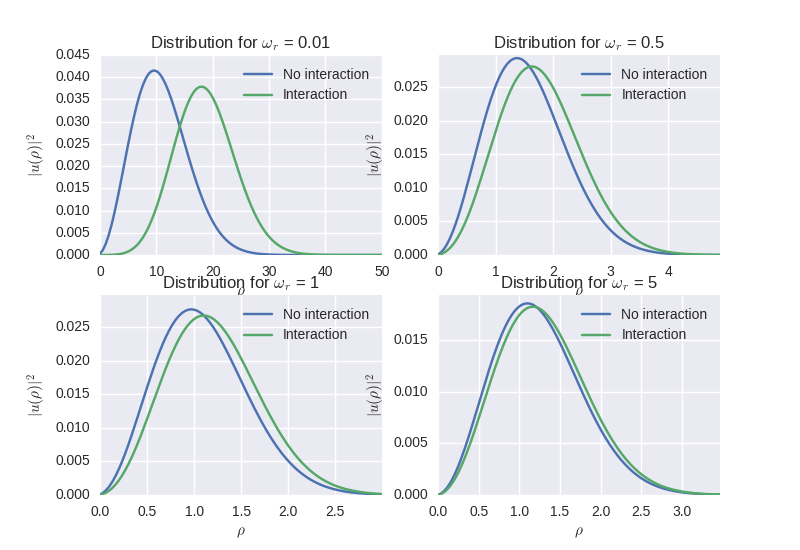
\includegraphics[scale=0.6]{distribution_subplot.png}\label{fig:finfigur}
\caption{Plots showing the probability distribution for the relative position of the two electrons. $\omega_r$ corresponds to the frequency of the harmonic oscillator potential, which can be seen as the width of the potential well.}
\end{figure}
\end{center}

\section{Discussion}
We have plotted the absolute value of the wavefunction (eigenvector of the ground state) squared. As our eigenvectors are normalized, this measures the probability of an electron to be at a specified position interval. Notice how $|u(\rho)|^{2}$ is more smeared out for a lower $\omega_r$ (takes on larger values). Notice further how the interacting and non-interacting cases are close at high $\omega_r$, but far apart at lower $\omega_r$.   We can interpret these results by considering the different potentials more closely.
\subsection{The non-interacting case}

In the non-interacting case the only potenial energy is the harmonic oscillator potential. In this case, as earlier noted, $\omega_r$ determines the width of the potential well, and therefore determines the probability of the relative distance for the electron: the greater $\omega$ is, the narrower the potential well. Consequently, the probability of the electrons being close is high. This corresponds excellently with our results.

\subsection{The interacting case}

It the interacting case, the harmonic oscillator and the Coloumb potential are competing.If we look at the two parts of the potential, we can see that for small $\rho$, the Coloums potential is dominant, whereas for larger $\rho$, the HO is dominant. By equating the expression for the potentials, we find that the domain where the Coloumb potential dominates is:

$$
\rho < \omega_r^{-\frac{1}{3}}
$$ 

Thus a smaller $\omega_r$ implies a larger domain where the Coloumb potential dominates. We therefore expect the relative distance between the two electrons to be relatively larger. This is exactly what can be seen from the results. For the larger $\omega$'s the HO well is quite narrow, and it is therefor wholly dominant, causing the solutions for both potentials to be similar. For smaller $\omega$'s the HO well is wider and the electrons can move further apart.
\section{Conclusion and outlook}
\subsection{Conclusion}
We have investigated the solution to Schroedinger's equation for two electrons in two separate potentials. The results seem consistent with our intuition of the system, and also appear to be numerically stable, as we saw from our trial and error investigation of the step size. Though it may be possible to investigate a larger span of $\omega_r$, we seem to have captured the general behavior for both the regime where the HO potential is significant and the regime where the Coloumb interaction is most significant.\\
\linebreak
\subsection{Outlook}
There is still much future work to be made.One could investigate the potential for multiple electrons (though this would be significantly more complicated). Another alternative would be to investigate a periodic potential, where the electron can jump between the wells. Furthermore, one could compare the computed solution to an analytic solution, such as the one found in \cite{Analytic}.
\begin{thebibliography}{9}
\bibitem{Quantum-Dots}
Loss, Daniel and DiVincenzo, David.
\textit{Quantum computation with quantum dots}
Phys. Rev. A 57, 120, 1998
\\\texttt{http://journals.aps.org/pra/abstract/10.1103/PhysRevA.57.120}

\bibitem{Morten}
Hjorth-Jensen, Morten.
\textit{Project2 - 2016}
Computational Physics Autumn 2016.
\\\texttt{https://github.com/CompPhysics/ComputationalPhysics/blob/gh-pages/doc/Projects}

\bibitem{Morten2}
Hjorth-Jensen, Morten.
\textit{Computational Physics Lectures: Linear Algebra methods }
Computational Physics Autumn 2016.
\\\texttt{http://compphysics.github.io/ComputationalPhysics/doc/pub/linalg/html/linalg.html}

\bibitem{Analytic}
Taut, M.
\textit{Two electrons in an external oscillator potential: Particular analytic solutions of a Coulomb correlation problem}
Phys. Rev. A 48, 3561, 1993
\\\texttt{http://journals.aps.org/pra/abstract/10.1103/PhysRevA.48.3561}





\end{thebibliography}

\end{document}

